\chapter{Implementation}

\section{Structure}
Based on the project algorithm design, its Java implementation unit complies with the specified structure and thus maintain the two core phases ($Analyse$ and $Generate$). However, hard code requires extra handling of data input and output. Hence additional two phases are added: $Scan$ and $Monitor$, which read and display input respectively. Moreover, the differences in data type of different iterations require extra treatment would be too clunky to append to the $Analyse$ phase. Thus, another phase is in line: $Sub-Analyse$, which inherits $Analyse$ range-analysing functions while having additional threshold check (for density) and handle elimination round for partly-covered tuples.  

The implementation process can now be divided into five Phases instead of two from the original algorithm. The reasoning is assessed in details below:

\begin{table}[!htbp]
\caption{5-Phase Implementation and Reasoning}
\label{table:table4_6}
\centering
\begin{tabular}{lc}
	\toprule
	\textbf{Reason} & \textbf{Outcome} \\
	\midrule
	To read and pre-process data input before
analysis & Phase I Scan \\
	To comply with the original structure	& Phase II Analyse \\
	To comply with the original structure	& Phase II Generate \\
	To adapt to different iteration needs	during
data analysing process & Phase IV Sub-Analyse \\
	To monitor and record the result & Phase V Monitor \\
	\bottomrule
\end{tabular} 
\end{table}



Details will be discussed in sections below for each phase. To demonstrate the structure visually, a Class Diagram and an Activity Diagram is shown for each phase, that is represented by each class. Reason is because Class Diagram is the most common representation for an overview within and between classes [SRC]. A Sequence Diagram could have been an alternative to Activity Diagram; however, Sequence Diagram fails to demonstrate the actual data flow as the programme needs to call different functions or initialise different objects in different iteration. It means the sequences between classes change depending on which round the programme is on, thus not shown accurately in one data flow chart as in Sequence Diagram [SRC]. Therefore, to demonstrate the purpose of classes, Activity Diagram is in use.

\subsection{Phase I Scan}

\begin{description}

\item[Aim: ] There are three aims within this phase or class:
\begin{itemize}
	\item{To read data from .csv file} 
	\item{To sort data into sub-data pools using class values found when reading data in} 
	\item{To pass these data into the next phase or class ($Analyser$} 
\end{itemize}

\item[Input: ] Assumed pre-processed csv file i.e. no null values within attributes and the order of element in an instance is {attribute 1, attribute 2,..., attribute N, class C}

\textit{Reason: } Initial plan included an extra processing unit for filtering csv file when value is Null. However, time constraint did not allow the construction of this unit. Hence the programme only consider pre-processed csv data at the time the report is written.

\item[Output: ] A list of all instances of the data - a list of tuples that are presented as lists ($AllTuples$). Moreover, a partitioned map that contains class values as keys that are connected to their relevant sub-data (list of instances) as values ($AllClassMap$)
  
\textit{Reason: } $AllTuples$ is required to provide access to all original data. $AllClassMap$ is required to get the class-based data partition since the key efficiency of this algorithm is to `divide and conquer' on data partitions guided by class tag [SRC]

\item[Data type: ] \texttt{LinkedList} (for tuples), \texttt{LinkedHashMap} (for class-based data partitioned map)

\textit{Reason: } A \texttt{List} (without specified inner data type) is used for tuples since it needs multiple types of data (e.g. float number, string class value, integer order). In this case, \texttt{LinkedList} is used instead of \texttt{ArrayList} due to its ability to add and remove first and last elements more quickly than the alternative [SRC]. It is necessary to retrieve class value at faster rate as class value is the last element in the tuple.

Similarly, a \texttt{LinkedHashMap} is used for faster retrieval rate in later parts. A \texttt{HashMap} is used for storing partitioned sub-data from class values since each partition of data needs to be recorded with its unique class value. It has String class as key and \texttt{LinkedList<LinkedList>} List of all tuples as values. 

\item[Class diagram: ] 

Its class diagram is in Figure 4.1, showing two features:
\begin{itemize}
	\item{scanData()} \\
	This method initialises two scanners, one to scan line-by-line data from csv file (i.e. tuples) and one to scan in-line elements (i.e. attributes).
	It processes data into 1) allTuple (where all instances are recorded from the first scanner) and 2) Class values, Tuple order numbering and Tuple attributes (which is sorted by the second scanners).
	The Class values become the parameter for the next method, where it helps create the Map that connects Class value to relevant set of Tuples.
	\item{sortData()} \\
	This method groups sets of tuples according to their Class value by checking their last String element. It sorts and partitions allTuple into sub-data pools, which are then passed on as parameter to the new class ($Analyser$).
	
\end{itemize}

\begin{figure}[!htbp]
    \centering
    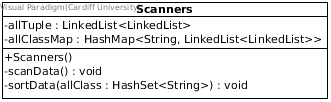
\includegraphics[width=4in]{figures/class_scanners}
    \caption[A Class Diagram for Phase I Scanners]{A Class Diagram for Phase I Scanners}
    \label{fig:figure4_1}
\end{figure}

\item[Activity diagram: ] 

FIG PLS

\end{description}

\subsection{Phase II Analyse}

\begin{description}

\item[Aim: ] Being the core module of the programme, there are important aims for this phase or class:
\begin{itemize}
	\item{To find (min, max) range for each attribute from class-based map.} 
	\item{To convert (min, max) range to binary array, which is ready for max-sum analysis.} 
	\item{To perform max-sum analysis on (min, max), aim to obtain at least one sub-optimal range, which is ready for the threshold test.} 
	\item{To perform threshold check. As discussed, this check diverses depending on which iteration. However, support and confidence is always required thus appear in this phase or class.} 
	\item{To modify the new sub-data pools for the next iteration. Since data set would shrink after pruning process from max-sum and (if applicable) strict-adjust method, current data set is frequently changing. Threshold measures, however, are calculated depending on these sets, thus makes this modification step necessary.} 
	\item{To pass the modified sub-data pools as well as new sub-ranges to the next phase or class ($Generator$).} 
\end{itemize}

WE ARE HERE

\item[Input: ] Assumed pre-processed csv file i.e. no null values within attributes and the order of element in an instance is {attribute 1, attribute 2,..., attribute N, class C}

\textit{Reason: } Initial plan included an extra processing unit for filtering csv file when value is Null. However, time constraint did not allow the construction of this unit. Hence the programme only consider pre-processed csv data at the time the report is written.

\item[Output: ] A list of all instances of the data - a list of tuples that are presented as lists ($AllTuples$). Moreover, a partitioned map that contains class values as keys that are connected to their relevant sub-data (list of instances) as values ($AllClassMap$)
  
\textit{Reason: } $AllTuples$ is required to provide access to all original data. $AllClassMap$ is required to get the class-based data partition since the key efficiency of this algorithm is to `divide and conquer' on data partitions guided by class tag [SRC]

\item[Data type: ] \texttt{LinkedList} (for tuples), \texttt{LinkedHashMap} (for class-based data partitioned map)

\textit{Reason: } A \texttt{List} (without specified inner data type) is used for tuples since it needs multiple types of data (e.g. float number, string class value, integer order). In this case, \texttt{LinkedList} is used instead of \texttt{ArrayList} due to its ability to add and remove first and last elements more quickly than the alternative [SRC]. It is necessary to retrieve class value at faster rate as class value is the last element in the tuple.

Similarly, a \texttt{LinkedHashMap} is used for faster retrieval rate in later parts. A \texttt{HashMap} is used for storing partitioned sub-data from class values since each partition of data needs to be recorded with its unique class value. It has String class as key and \texttt{LinkedList<LinkedList>} List of all tuples as values. 

\item[Class diagram: ] 

Its class diagram is in Figure 4.1, showing two features:
\begin{itemize}
	\item scanData()
	This method initialises two scanners, one to scan line-by-line data from csv file (i.e. tuples) and one to scan in-line elements (i.e. attributes).
	It processes data into 1) allTuple (where all instances are recorded from the first scanner) and 2) Class values, Tuple order numbering and Tuple attributes (which is sorted by the second scanners).
	The Class values become the parameter for the next method, where it helps create the Map that connects Class value to relevant set of Tuples.
	\item sortData()
	This method groups sets of tuples according to their Class value by checking their last String element. It sorts and partitions allTuple into sub-data pools, which are then passed on as parameter to the new class ($Analyser$).
	
\end{itemize}

\begin{figure}[t]
    \centering
    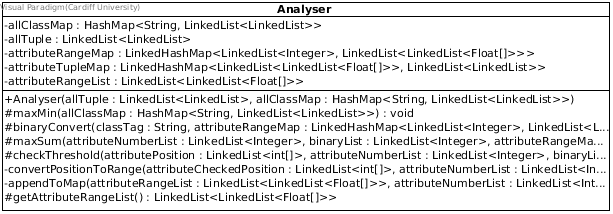
\includegraphics[width=5in]{figures/class_analyser}
    \caption[A Class Diagram for Phase II Analyser]{A Class Diagram for Phase II Analyser}
    \label{fig:figure4_2}
\end{figure}

\item[Activity diagram: ] 
\end{description}





